%------------------------
% Ethan's Résumé Template
% Author: necusjz
% License: CC-BY-4.0
%------------------------
\documentclass[letterpaper,11pt]{article}

\usepackage{latexsym}
\usepackage[empty]{fullpage}
\usepackage{titlesec}
\usepackage{marvosym}
\usepackage[usenames,dvipsnames]{color}
\usepackage{verbatim}
\usepackage{enumitem}
\usepackage[hidelinks]{hyperref}
\usepackage{fancyhdr}
\usepackage[english]{babel}
\usepackage{tabularx}
\usepackage{fontawesome5}
\usepackage{ragged2e}
\usepackage{etoolbox}
\usepackage{tikz}
\input{glyphtounicode}

% font options
\usepackage[sc]{mathpazo}
\linespread{1.05}  % palladio needs more leading (space between lines)
\usepackage[T1]{fontenc}

\pagestyle{fancy}
\fancyhf{}  % clear all header and footer fields
\fancyfoot{}
\renewcommand{\headrulewidth}{0pt}
\renewcommand{\footrulewidth}{0pt}
\usepackage{float}

% adjust margins
\addtolength{\oddsidemargin}{-0.5in}
\addtolength{\evensidemargin}{-0.5in}
\addtolength{\textwidth}{1in}
\addtolength{\topmargin}{-.5in}
\addtolength{\textheight}{1.0in}

\urlstyle{same}

\raggedbottom
\raggedright
\setlength{\tabcolsep}{0in}
\setlength{\footskip}{5pt}

% sections formatting
\titleformat{\section}{
  \vspace{-4pt}\scshape\raggedright\large
}{}{0em}{}[\color{black}\titlerule \vspace{-5pt}]

% ensure that generate pdf is machine readable/ATS parsable
\pdfgentounicode=1

% custom commands
\newcommand{\cvitem}[1]{
  \item\small{
    {#1\vspace{-2pt}}
  }
}

\newcommand{\cvheading}[4]{
  \vspace{-2pt}\item
    \begin{tabular*}{\textwidth}[t]{l@{\extracolsep{\fill}}r}
      \textbf{#1} & #2 \\
      \small#3 & \small #4 \\
    \end{tabular*}\vspace{-7pt}
}

\newcommand{\cvheadingstart}{\begin{itemize}[leftmargin=0in, label={}]}
\newcommand{\cvheadingend}{\end{itemize}}
\newcommand{\cvitemstart}{\begin{itemize}\justifying}
\newcommand{\cvitemend}{\end{itemize}\vspace{-5pt}}

\newcommand{\cvskill}[2]{
  \textcolor{black}{\textbf{#1}}\hfill
  \foreach \x in {1,...,5}{%
    \space{\ifnumgreater{\x}{#2}{\color{black!80!white!20}}{\color{black}}\faSquare}}\par%
  \vspace{-2pt}
}

\renewcommand\labelitemii{$\vcenter{\hbox{\footnotesize$\bullet$}}$}

\begin{document}

% contact information
\begin{center}
  \textbf{\LARGE\scshape PG-Sheets Template (Name of your dataset)} \\
  \vspace{1pt}\small
\end{center}

\section{Instructions on PG-Sheets}
PG-Sheets is a document composed of questions that can be used as guidelines for documenting Property Graph datasets. 
The PG-Sheets sections and questions are inspired by the 5W1H (Who, What, Where, When, Why, and How) writing technique, in which each section should answer one of the questions What? Where? When? Why? and How? about the data, and the answer to Who? is embedded in each section. The overarching hypothesis behind PG-Sheets is that if a dataset’s documentation successfully addresses all these questions, then it can be considered complete and concise.

Each PG-Sheet is intended to provide all the essential information a reader or potential data user needs to understand the dataset, including its strengths, limitations, and context of use.
Each one of the sections has a set of questions which is labeled according to the following priority level:
\begin{itemize}
    \item \textcolor{red}{MUST} - questions that must always be answered and included in a PG-Sheet. 
    \item \textcolor{yellow}{SHOULD} - questions that should be answered, but are not mandatory to have.
    \item \textcolor{green}{NICE} - questions that would be nice to have an answer but can be considered optional. 
\end{itemize}

This template presents each question along with recommendations or expected answer formats. These should be treated as guidelines and adapted to the context of the specific property graph dataset being documented.

\section{Executive Summary \textcolor{red}{(MUST)}}

This section can be considered an abstract of your documentation; it contains the basic information about your dataset. 

\begin{table}[htb]\color{red}
\centering
\small\begin{tabular}{|l|l|}
\hline
Dataset Name & name of the dataset \\ \hline
Number of Node Labels & - \\ \hline
Number of Edge Labels & - \\ \hline
Total number of nodes & - \\ \hline
Total number of edges & - \\ \hline
Version & - \\ \hline
Source & - \\ \hline
Dataset authors & - \\ \hline
How to cite & - \\ \hline
PG-Sheets authors & -  \\ \hline
\end{tabular}
\end{table}

\section{Composition (What?)}

\textbf{\textcolor{red}{Context/Domain of the data (MUST)}} - What is the domain of the data and its context? For example, if the dataset is part of the biomedical domain, financial data, temporal information, and the general context of the data. 

\textbf{\textcolor{red}{Information about the instances (MUST) }} - Schema information about the property graph (entities, labels, properties, and its type). Here the schema of the graph should be exposed in two different ways: (1) graphical way as a figure that contains nodes and edge labels, the attributes of each label and its data type, and the connections every two nodes can have (see example \autoref{fig:enter-label}), and (2) in a tabular format which contains the same information but in a tabular format for ease of understanding. The answer should also include who made the schema and who wrote the information in the PG-Sheet. % → Schema information about the property graph (entities, labels, properties, and their type)

\begin{figure}
    \centering
    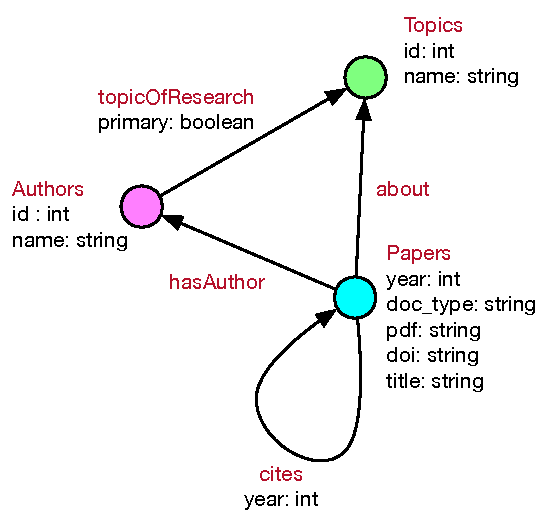
\includegraphics[width=0.4\linewidth]{pgsheetsExampleSchema.pdf}
    \caption{Example of a property graph schema figure}
    \label{fig:enter-label}
\end{figure}


\begin{table}[H]
\centering
\footnotesize
\begin{tabular}{|l|l|l|}
\hline
Label                            & Attribute/Property       & Description                                                  \\ \hline
Node or edge label (e.g. Person) & Property key (e.g. name) & Natural language description of what this property refers to \\ \hline
                                 &                          &                                                              \\ \hline
\end{tabular}
\caption{Table with description of the properties}
\end{table}

\begin{minipage}{0.48\textwidth}
\centering
\footnotesize
\begin{tabular}{|l|l|}
\hline
Node Label         & Size                            \\ \hline
Node (e.g. Authors) & Number of nodes labelled Authors \\ \hline
                   &                                 \\ \hline
\end{tabular}
\end{minipage}%
\hfill
\begin{minipage}{0.48\textwidth}
\centering
\footnotesize
\begin{tabular}{|l|l|}
\hline
Edge Label        & Size                           \\ \hline
Edge (e.g. about) & Number of edges labelled about \\ \hline
                  &                                \\ \hline
\end{tabular}
\end{minipage}

\textbf{\textcolor{red}{Important additional information (MUST)}} - This section should contain additional important information about the graph schema. This additional information includes a known distribution/range of values of considered important attributes, constraints, and semantic information. These should be described in this document in a natural language format or, in the case of value distribution, using plots and exposing it as a figure. 
In case information about constraints is available in a specific language (e.g. PG-Keys), it should be added as a separate file in the repository and referenced in PG-Sheets, however, there must always be a natural language explanation for each constraint referenced in the PG-Sheets document. 

Who detected or wrote about each of the additional information should also be indicated in this section. Why such constraints/information is important and in which context needs to be included in this answer as well. 

%- about the data such as distribution/range of values, are the IDs unique, semantic information, etc
\textbf{\textcolor{red}{Does it rely on external sources? (MUST)}} - Was the property graph generated according to an external source? Or does the composition of the graph rely on a third-party system? Who and why this choice was made.
Essentially in this question, we want to know if the dataset is generated, for example, according to an external source or tool that might change the content of the data).

\textbf{\textcolor{red}{Dataset splits or other samples available in the repository that contains this same data or the other way around (MUST)}} - point to other splits or samples of the same data in the repository, declare if the schema is the same or not. Who made the split and why this decision was made. More details about the collection aspects should be declared in the data collection section. 

\textbf{\textcolor{red}{How is it different from other versions? (MUST)}}
If the answer to the previous question is yes, then this answer should be declared what is different from its split. 

\section{Motivation (Why?)}

\textbf{\textcolor{red}{Why was the dataset created? (MUST)}} - What is the motivation behind the creation of this dataset? Does this dataset have specific characteristics that previous datasets for the same task did not cover? 

\textbf{\textcolor{red}{Which task was it intended to solve? (MUST)}} - What kind of problem was it intended to solve, e.g., frequent subgraph mining, path query evaluation, entity linking, etc. Why was this type of data/domain collected to solve this task?

\textbf{\textcolor{red}{Has this data been used before? (MUST)}} If yes, give examples or links to where it was used - if it is a sample of previous data, specify it in the data collection section
Similar to the question in the composition section but from the perspective of why this data was sampled or split into another dataset. 

\textbf{\textcolor{red}{If it has been used or is a sample, why was each of the entities chosen? (MUST)}}


\textbf{\textcolor{red}{Reasoning behind the modeling of the graph (MUST)}} - Why the dataset/graph was modeled in the way that it was exposed in the Composition section of the paper. 

\section{Data Collection and Pre-processing (When? How?)}

\textbf{\textcolor{red}{Source of data (MUST)}} - If it is collected from sensors or other appliances, this question should describe the hardware specification. If the data was collected from a website, it should include a link and description of the website. %(hardware, link to other website) 

\textbf{\textcolor{red}{Time-frame that the data was collected (MUST)}} Dates in which the collection and processing of the data were made.
\textbf{\textcolor{red}{How the dataset was collected? (MUST)}} This question includes which method was used to collect the dataset and what kind of pre-processing was applied to this data including who was responsible for each part of the data collection and processing phase and why each method was applied to get to the final dataset. Here we recommend using figures to explain the different steps and methods applied. The figure should be clear enough to understand the many steps used in the property graph dataset construction process. %method used) and which preprocessing steps were done (and why)

\textbf{\textcolor{red}{Is the dataset a sample? (MUST)}} If yes, include information about the full dataset, similar to the previous information. %(information about the full dataset)

\textbf{\textcolor{red}{Who is involved in each one of the collection steps? (MUST)}} can be answered together with the collection steps questions. 

\textbf{\textcolor{yellow}{Is the raw data available? (SHOULD)}} (if there is any) - is the raw data of this dataset (without any processing steps post data collection) available for access, if yes, include the link to the webpage. 

\textbf{\textcolor{yellow}{Method used for collection available? (SHOULD)}} (external software for example) - IF the collection method was done by a software, link the software on this page. 

\section{Distribution and Maintenance (Where?)}

\begin{table}[htb]
\begin{tabular}{|l|l|}
\hline
\textcolor{red}{License of the dataset (MUST)} & - \\ \hline
\textcolor{red}{Date of Distribution (MUST)} & -  \\ \hline
\textcolor{red}{Dates of Modification (MUST)} & Maintenance dates and how did it change in each version \\ \hline
\textcolor{red}{Responsible for hosting the dataset (MUST)} & Institution or name of the person responsible\\ \hline
\textcolor{red}{Responsible for maintaining the dataset (MUST)} &  Contact of who is maintaining the dataset\\ \hline
\end{tabular}
\end{table}

\textbf{\textcolor{green}{Papers that use this dataset? (NICE)}} → Link to any publicly available information, for example, papers and references that use the same data. 

\textbf{\textcolor{green}{How can a third party contribute to this dataset? (NICE}} - Instructions on how to contribute to the dataset and who is the person in contact in this case.

\textbf{\textcolor{green}{Additional Comments (NICE)}} - Additional comments regarding the license or distribution of this dataset (e.g. cannot be distributed on other platforms without the consent of the authors)

\section{Using the dataset and legal/ethical aspects (How?)}

\textbf{\textcolor{red}{Was this dataset approved by an ethical review? (MUST)}} - If yes, link to the ethical review it was approved from to a page that contains information about the ethical review it was submitted to. 


\textbf{\textcolor{red}{Privacy issues (MUST)}}  (if this was part of the data preprocessing - explain what were the privacy related risks that the raw data contained) - are there any attributes or data that have to be anonymized? And if yes then make it clear also in the preprocessing step. If not, then answer why privacy is not an issue in this dataset. 


\textbf{\textcolor{red}{Ethical issues (MUST)}} → does it advantage or disadvantage a specific group? If this is unknown, give an overview of the known groups in this data so users know which are the potential groups that they should look into

\textbf{\textcolor{red}{Does it contain inappropriate information? Or any potentially inappropriate data? (MUST)}} - If it is not known, declare it in this question. 

\textbf{\textcolor{red}{Does it comply with a data protection regulation law? (MUST)}} e.g. GDPR, or similar from another country?


\textbf{\textcolor{red}{How to use the dataset? (MUST)}} (Instructions on loading the dataset/external software that can be used, etc)

\end{document}
